% !TEX TS-program = pdflatex
% !TEX encoding = UTF-8 Unicode
\documentclass[border=0mm]{standalone}
% packages
\usepackage{tikz}
\usetikzlibrary{patterns}
\usepackage{amsmath,amssymb}
\usepackage{bm}
\usepackage{pgfplots}
\pgfplotsset{compat=1.15}
% start document
\begin{document}
% generated by ROOT (CERN)
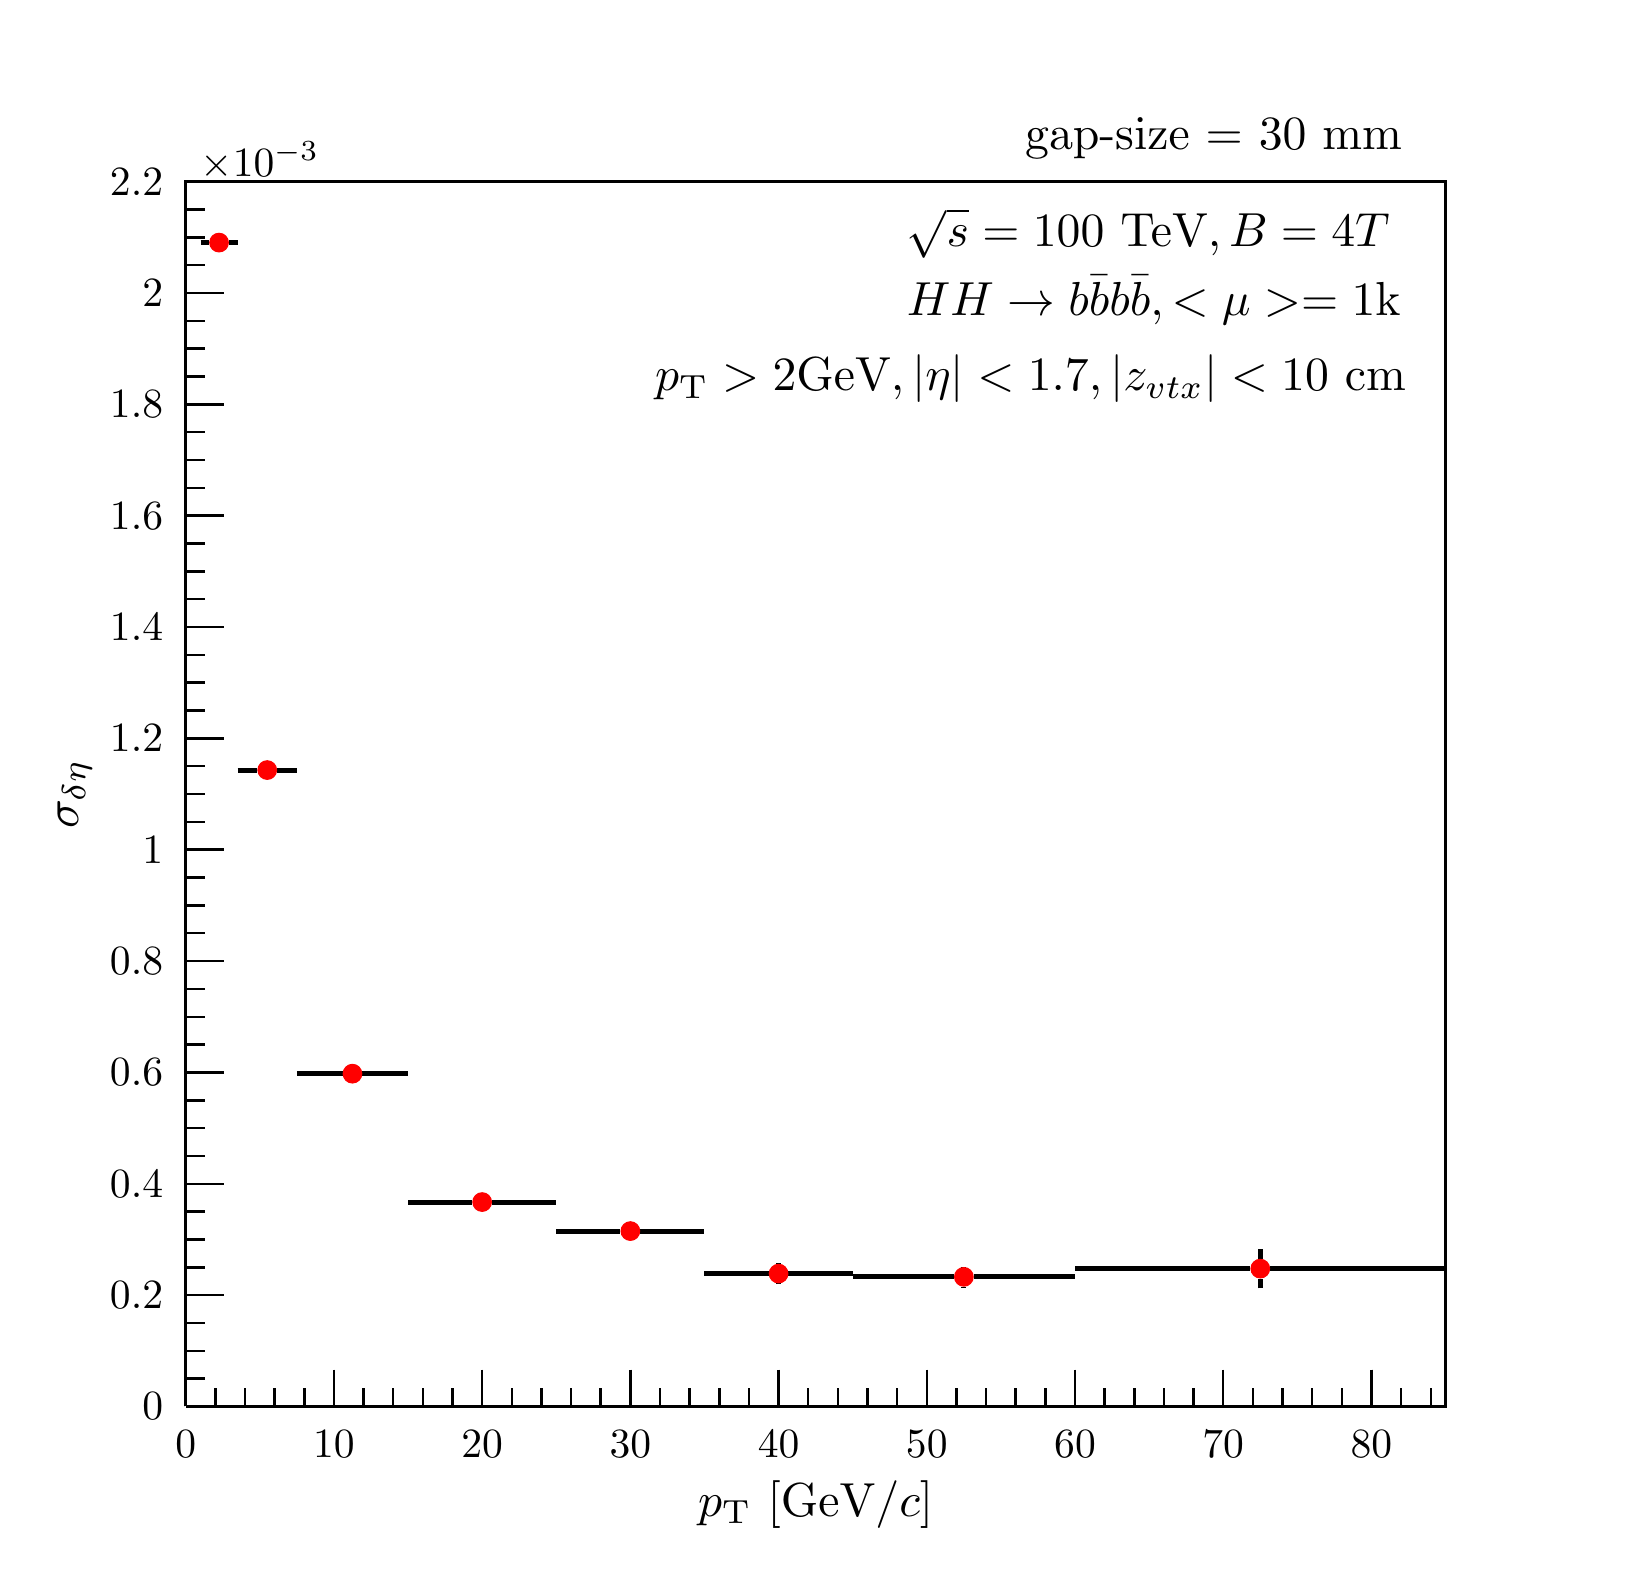
\begin{tikzpicture}
\pgfdeclareplotmark{cross} {
\pgfpathmoveto{\pgfpoint{-0.3\pgfplotmarksize}{\pgfplotmarksize}}
\pgfpathlineto{\pgfpoint{+0.3\pgfplotmarksize}{\pgfplotmarksize}}
\pgfpathlineto{\pgfpoint{+0.3\pgfplotmarksize}{0.3\pgfplotmarksize}}
\pgfpathlineto{\pgfpoint{+1\pgfplotmarksize}{0.3\pgfplotmarksize}}
\pgfpathlineto{\pgfpoint{+1\pgfplotmarksize}{-0.3\pgfplotmarksize}}
\pgfpathlineto{\pgfpoint{+0.3\pgfplotmarksize}{-0.3\pgfplotmarksize}}
\pgfpathlineto{\pgfpoint{+0.3\pgfplotmarksize}{-1.\pgfplotmarksize}}
\pgfpathlineto{\pgfpoint{-0.3\pgfplotmarksize}{-1.\pgfplotmarksize}}
\pgfpathlineto{\pgfpoint{-0.3\pgfplotmarksize}{-0.3\pgfplotmarksize}}
\pgfpathlineto{\pgfpoint{-1.\pgfplotmarksize}{-0.3\pgfplotmarksize}}
\pgfpathlineto{\pgfpoint{-1.\pgfplotmarksize}{0.3\pgfplotmarksize}}
\pgfpathlineto{\pgfpoint{-0.3\pgfplotmarksize}{0.3\pgfplotmarksize}}
\pgfpathclose
\pgfusepathqstroke
}
\pgfdeclareplotmark{cross*} {
\pgfpathmoveto{\pgfpoint{-0.3\pgfplotmarksize}{\pgfplotmarksize}}
\pgfpathlineto{\pgfpoint{+0.3\pgfplotmarksize}{\pgfplotmarksize}}
\pgfpathlineto{\pgfpoint{+0.3\pgfplotmarksize}{0.3\pgfplotmarksize}}
\pgfpathlineto{\pgfpoint{+1\pgfplotmarksize}{0.3\pgfplotmarksize}}
\pgfpathlineto{\pgfpoint{+1\pgfplotmarksize}{-0.3\pgfplotmarksize}}
\pgfpathlineto{\pgfpoint{+0.3\pgfplotmarksize}{-0.3\pgfplotmarksize}}
\pgfpathlineto{\pgfpoint{+0.3\pgfplotmarksize}{-1.\pgfplotmarksize}}
\pgfpathlineto{\pgfpoint{-0.3\pgfplotmarksize}{-1.\pgfplotmarksize}}
\pgfpathlineto{\pgfpoint{-0.3\pgfplotmarksize}{-0.3\pgfplotmarksize}}
\pgfpathlineto{\pgfpoint{-1.\pgfplotmarksize}{-0.3\pgfplotmarksize}}
\pgfpathlineto{\pgfpoint{-1.\pgfplotmarksize}{0.3\pgfplotmarksize}}
\pgfpathlineto{\pgfpoint{-0.3\pgfplotmarksize}{0.3\pgfplotmarksize}}
\pgfpathclose
\pgfusepathqfillstroke
}
\pgfdeclareplotmark{newstar} {
\pgfpathmoveto{\pgfqpoint{0pt}{\pgfplotmarksize}}
\pgfpathlineto{\pgfqpointpolar{44}{0.5\pgfplotmarksize}}
\pgfpathlineto{\pgfqpointpolar{18}{\pgfplotmarksize}}
\pgfpathlineto{\pgfqpointpolar{-20}{0.5\pgfplotmarksize}}
\pgfpathlineto{\pgfqpointpolar{-54}{\pgfplotmarksize}}
\pgfpathlineto{\pgfqpointpolar{-90}{0.5\pgfplotmarksize}}
\pgfpathlineto{\pgfqpointpolar{234}{\pgfplotmarksize}}
\pgfpathlineto{\pgfqpointpolar{198}{0.5\pgfplotmarksize}}
\pgfpathlineto{\pgfqpointpolar{162}{\pgfplotmarksize}}
\pgfpathlineto{\pgfqpointpolar{134}{0.5\pgfplotmarksize}}
\pgfpathclose
\pgfusepathqstroke
}
\pgfdeclareplotmark{newstar*} {
\pgfpathmoveto{\pgfqpoint{0pt}{\pgfplotmarksize}}
\pgfpathlineto{\pgfqpointpolar{44}{0.5\pgfplotmarksize}}
\pgfpathlineto{\pgfqpointpolar{18}{\pgfplotmarksize}}
\pgfpathlineto{\pgfqpointpolar{-20}{0.5\pgfplotmarksize}}
\pgfpathlineto{\pgfqpointpolar{-54}{\pgfplotmarksize}}
\pgfpathlineto{\pgfqpointpolar{-90}{0.5\pgfplotmarksize}}
\pgfpathlineto{\pgfqpointpolar{234}{\pgfplotmarksize}}
\pgfpathlineto{\pgfqpointpolar{198}{0.5\pgfplotmarksize}}
\pgfpathlineto{\pgfqpointpolar{162}{\pgfplotmarksize}}
\pgfpathlineto{\pgfqpointpolar{134}{0.5\pgfplotmarksize}}
\pgfpathclose
\pgfusepathqfillstroke
}
\definecolor{c}{rgb}{1,1,1};
\draw [color=c, fill=c] (0,0) rectangle (20,19.4486);
\draw [color=c, fill=c] (2,1.94486) rectangle (18,17.5038);
\definecolor{c}{rgb}{0,0,0};
\draw [c,line width=0.9] (2,1.94486) -- (2,17.5038) -- (18,17.5038) -- (18,1.94486) -- (2,1.94486);
\definecolor{c}{rgb}{1,1,1};
\draw [color=c, fill=c] (2,1.94486) rectangle (18,17.5038);
\definecolor{c}{rgb}{0,0,0};
\draw [c,line width=0.9] (2,1.94486) -- (2,17.5038) -- (18,17.5038) -- (18,1.94486) -- (2,1.94486);
\draw [c,line width=1.8] (2.18824,16.7259) -- (2.29822,16.7259);
\draw [c,line width=1.8] (2.54884,16.7259) -- (2.65882,16.7259);
\definecolor{c}{rgb}{1,0,0};
\foreach \P in {(2.42353,16.7259)}{\draw[mark options={color=c,fill=c},mark size=3.363363pt,mark=*] plot coordinates {\P};}
\definecolor{c}{rgb}{0,0,0};
\draw [c,line width=1.8] (2.65882,10.0271) -- (2.90998,10.0271);
\draw [c,line width=1.8] (3.16061,10.0271) -- (3.41176,10.0271);
\definecolor{c}{rgb}{1,0,0};
\foreach \P in {(3.03529,10.0271)}{\draw[mark options={color=c,fill=c},mark size=3.363363pt,mark=*] plot coordinates {\P};}
\definecolor{c}{rgb}{0,0,0};
\draw [c,line width=1.8] (3.41176,6.17129) -- (3.99233,6.17129);
\draw [c,line width=1.8] (4.24296,6.17129) -- (4.82353,6.17129);
\definecolor{c}{rgb}{1,0,0};
\foreach \P in {(4.11765,6.17129)}{\draw[mark options={color=c,fill=c},mark size=3.363363pt,mark=*] plot coordinates {\P};}
\definecolor{c}{rgb}{0,0,0};
\draw [c,line width=1.8] (4.82353,4.54094) -- (5.63939,4.54094);
\draw [c,line width=1.8] (5.89002,4.54094) -- (6.70588,4.54094);
\definecolor{c}{rgb}{1,0,0};
\foreach \P in {(5.76471,4.54094)}{\draw[mark options={color=c,fill=c},mark size=3.363363pt,mark=*] plot coordinates {\P};}
\definecolor{c}{rgb}{0,0,0};
\draw [c,line width=1.8] (6.70588,4.17228) -- (7.52175,4.17228);
\draw [c,line width=1.8] (7.77237,4.17228) -- (8.58823,4.17228);
\definecolor{c}{rgb}{1,0,0};
\foreach \P in {(7.64706,4.17228)}{\draw[mark options={color=c,fill=c},mark size=3.363363pt,mark=*] plot coordinates {\P};}
\definecolor{c}{rgb}{0,0,0};
\draw [c,line width=1.8] (9.52941,3.49802) -- (9.52941,3.50686);
\draw [c,line width=1.8] (9.52941,3.75748) -- (9.52941,3.76632);
\draw [c,line width=1.8] (8.58823,3.63217) -- (9.4041,3.63217);
\draw [c,line width=1.8] (9.65473,3.63217) -- (10.4706,3.63217);
\definecolor{c}{rgb}{1,0,0};
\foreach \P in {(9.52941,3.63217)}{\draw[mark options={color=c,fill=c},mark size=3.363363pt,mark=*] plot coordinates {\P};}
\definecolor{c}{rgb}{0,0,0};
\draw [c,line width=1.8] (11.8824,3.46004) -- (11.8824,3.46552);
\draw [c,line width=1.8] (11.8824,3.71615) -- (11.8824,3.72163);
\draw [c,line width=1.8] (10.4706,3.59083) -- (11.757,3.59083);
\draw [c,line width=1.8] (12.0077,3.59083) -- (13.2941,3.59083);
\definecolor{c}{rgb}{1,0,0};
\foreach \P in {(11.8824,3.59083)}{\draw[mark options={color=c,fill=c},mark size=3.363363pt,mark=*] plot coordinates {\P};}
\definecolor{c}{rgb}{0,0,0};
\draw [c,line width=1.8] (15.6471,3.445) -- (15.6471,3.56993);
\draw [c,line width=1.8] (15.6471,3.82055) -- (15.6471,3.94548);
\draw [c,line width=1.8] (13.2941,3.69524) -- (15.5217,3.69524);
\draw [c,line width=1.8] (15.7724,3.69524) -- (18,3.69524);
\definecolor{c}{rgb}{1,0,0};
\foreach \P in {(15.6471,3.69524)}{\draw[mark options={color=c,fill=c},mark size=3.363363pt,mark=*] plot coordinates {\P};}
\definecolor{c}{rgb}{0,0,0};
\draw [c,line width=0.9] (2,1.94486) -- (18,1.94486);
\draw [c,line width=0.9] (2,2.41163) -- (2,1.94486);
\draw [c,line width=0.9] (2.37647,2.17825) -- (2.37647,1.94486);
\draw [c,line width=0.9] (2.75294,2.17825) -- (2.75294,1.94486);
\draw [c,line width=0.9] (3.12941,2.17825) -- (3.12941,1.94486);
\draw [c,line width=0.9] (3.50588,2.17825) -- (3.50588,1.94486);
\draw [c,line width=0.9] (3.88235,2.41163) -- (3.88235,1.94486);
\draw [c,line width=0.9] (4.25882,2.17825) -- (4.25882,1.94486);
\draw [c,line width=0.9] (4.63529,2.17825) -- (4.63529,1.94486);
\draw [c,line width=0.9] (5.01177,2.17825) -- (5.01177,1.94486);
\draw [c,line width=0.9] (5.38824,2.17825) -- (5.38824,1.94486);
\draw [c,line width=0.9] (5.76471,2.41163) -- (5.76471,1.94486);
\draw [c,line width=0.9] (6.14118,2.17825) -- (6.14118,1.94486);
\draw [c,line width=0.9] (6.51765,2.17825) -- (6.51765,1.94486);
\draw [c,line width=0.9] (6.89412,2.17825) -- (6.89412,1.94486);
\draw [c,line width=0.9] (7.27059,2.17825) -- (7.27059,1.94486);
\draw [c,line width=0.9] (7.64706,2.41163) -- (7.64706,1.94486);
\draw [c,line width=0.9] (8.02353,2.17825) -- (8.02353,1.94486);
\draw [c,line width=0.9] (8.4,2.17825) -- (8.4,1.94486);
\draw [c,line width=0.9] (8.77647,2.17825) -- (8.77647,1.94486);
\draw [c,line width=0.9] (9.15294,2.17825) -- (9.15294,1.94486);
\draw [c,line width=0.9] (9.52941,2.41163) -- (9.52941,1.94486);
\draw [c,line width=0.9] (9.90588,2.17825) -- (9.90588,1.94486);
\draw [c,line width=0.9] (10.2824,2.17825) -- (10.2824,1.94486);
\draw [c,line width=0.9] (10.6588,2.17825) -- (10.6588,1.94486);
\draw [c,line width=0.9] (11.0353,2.17825) -- (11.0353,1.94486);
\draw [c,line width=0.9] (11.4118,2.41163) -- (11.4118,1.94486);
\draw [c,line width=0.9] (11.7882,2.17825) -- (11.7882,1.94486);
\draw [c,line width=0.9] (12.1647,2.17825) -- (12.1647,1.94486);
\draw [c,line width=0.9] (12.5412,2.17825) -- (12.5412,1.94486);
\draw [c,line width=0.9] (12.9176,2.17825) -- (12.9176,1.94486);
\draw [c,line width=0.9] (13.2941,2.41163) -- (13.2941,1.94486);
\draw [c,line width=0.9] (13.6706,2.17825) -- (13.6706,1.94486);
\draw [c,line width=0.9] (14.0471,2.17825) -- (14.0471,1.94486);
\draw [c,line width=0.9] (14.4235,2.17825) -- (14.4235,1.94486);
\draw [c,line width=0.9] (14.8,2.17825) -- (14.8,1.94486);
\draw [c,line width=0.9] (15.1765,2.41163) -- (15.1765,1.94486);
\draw [c,line width=0.9] (15.5529,2.17825) -- (15.5529,1.94486);
\draw [c,line width=0.9] (15.9294,2.17825) -- (15.9294,1.94486);
\draw [c,line width=0.9] (16.3059,2.17825) -- (16.3059,1.94486);
\draw [c,line width=0.9] (16.6824,2.17825) -- (16.6824,1.94486);
\draw [c,line width=0.9] (17.0588,2.41163) -- (17.0588,1.94486);
\draw [c,line width=0.9] (17.0588,2.41163) -- (17.0588,1.94486);
\draw [c,line width=0.9] (17.4353,2.17825) -- (17.4353,1.94486);
\draw [c,line width=0.9] (17.8118,2.17825) -- (17.8118,1.94486);
\draw [anchor=base] (2,1.30306) node[scale=1.50291, color=c, rotate=0]{0};
\draw [anchor=base] (3.88235,1.30306) node[scale=1.50291, color=c, rotate=0]{10};
\draw [anchor=base] (5.76471,1.30306) node[scale=1.50291, color=c, rotate=0]{20};
\draw [anchor=base] (7.64706,1.30306) node[scale=1.50291, color=c, rotate=0]{30};
\draw [anchor=base] (9.52941,1.30306) node[scale=1.50291, color=c, rotate=0]{40};
\draw [anchor=base] (11.4118,1.30306) node[scale=1.50291, color=c, rotate=0]{50};
\draw [anchor=base] (13.2941,1.30306) node[scale=1.50291, color=c, rotate=0]{60};
\draw [anchor=base] (15.1765,1.30306) node[scale=1.50291, color=c, rotate=0]{70};
\draw [anchor=base] (17.0588,1.30306) node[scale=1.50291, color=c, rotate=0]{80};
\draw (10,0.700151) node[scale=1.72557, color=c, rotate=0]{$p_{\text{T}} ~[\text{GeV}/c]$};
\draw [c,line width=0.9] (2,1.94486) -- (2,17.5038);
\draw [c,line width=0.9] (2.48,1.94486) -- (2,1.94486);
\draw [c,line width=0.9] (2.24,2.29838) -- (2,2.29838);
\draw [c,line width=0.9] (2.24,2.65191) -- (2,2.65191);
\draw [c,line width=0.9] (2.24,3.00543) -- (2,3.00543);
\draw [c,line width=0.9] (2.48,3.35895) -- (2,3.35895);
\draw [c,line width=0.9] (2.24,3.71247) -- (2,3.71247);
\draw [c,line width=0.9] (2.24,4.06599) -- (2,4.06599);
\draw [c,line width=0.9] (2.24,4.41951) -- (2,4.41951);
\draw [c,line width=0.9] (2.48,4.77304) -- (2,4.77304);
\draw [c,line width=0.9] (2.24,5.12656) -- (2,5.12656);
\draw [c,line width=0.9] (2.24,5.48008) -- (2,5.48008);
\draw [c,line width=0.9] (2.24,5.8336) -- (2,5.8336);
\draw [c,line width=0.9] (2.48,6.18712) -- (2,6.18712);
\draw [c,line width=0.9] (2.24,6.54064) -- (2,6.54064);
\draw [c,line width=0.9] (2.24,6.89417) -- (2,6.89417);
\draw [c,line width=0.9] (2.24,7.24769) -- (2,7.24769);
\draw [c,line width=0.9] (2.48,7.60121) -- (2,7.60121);
\draw [c,line width=0.9] (2.24,7.95473) -- (2,7.95473);
\draw [c,line width=0.9] (2.24,8.30825) -- (2,8.30825);
\draw [c,line width=0.9] (2.24,8.66177) -- (2,8.66177);
\draw [c,line width=0.9] (2.48,9.0153) -- (2,9.0153);
\draw [c,line width=0.9] (2.24,9.36882) -- (2,9.36882);
\draw [c,line width=0.9] (2.24,9.72234) -- (2,9.72234);
\draw [c,line width=0.9] (2.24,10.0759) -- (2,10.0759);
\draw [c,line width=0.9] (2.48,10.4294) -- (2,10.4294);
\draw [c,line width=0.9] (2.24,10.7829) -- (2,10.7829);
\draw [c,line width=0.9] (2.24,11.1364) -- (2,11.1364);
\draw [c,line width=0.9] (2.24,11.4899) -- (2,11.4899);
\draw [c,line width=0.9] (2.48,11.8435) -- (2,11.8435);
\draw [c,line width=0.9] (2.24,12.197) -- (2,12.197);
\draw [c,line width=0.9] (2.24,12.5505) -- (2,12.5505);
\draw [c,line width=0.9] (2.24,12.904) -- (2,12.904);
\draw [c,line width=0.9] (2.48,13.2576) -- (2,13.2576);
\draw [c,line width=0.9] (2.24,13.6111) -- (2,13.6111);
\draw [c,line width=0.9] (2.24,13.9646) -- (2,13.9646);
\draw [c,line width=0.9] (2.24,14.3181) -- (2,14.3181);
\draw [c,line width=0.9] (2.48,14.6716) -- (2,14.6716);
\draw [c,line width=0.9] (2.24,15.0252) -- (2,15.0252);
\draw [c,line width=0.9] (2.24,15.3787) -- (2,15.3787);
\draw [c,line width=0.9] (2.24,15.7322) -- (2,15.7322);
\draw [c,line width=0.9] (2.48,16.0857) -- (2,16.0857);
\draw [c,line width=0.9] (2.24,16.4393) -- (2,16.4393);
\draw [c,line width=0.9] (2.24,16.7928) -- (2,16.7928);
\draw [c,line width=0.9] (2.24,17.1463) -- (2,17.1463);
\draw [c,line width=0.9] (2.48,17.4998) -- (2,17.4998);
\draw [c,line width=0.9] (2.48,17.4998) -- (2,17.4998);
\draw [anchor= east] (1.9,1.94486) node[scale=1.50291, color=c, rotate=0]{0};
\draw [anchor= east] (1.9,3.35895) node[scale=1.50291, color=c, rotate=0]{0.2};
\draw [anchor= east] (1.9,4.77304) node[scale=1.50291, color=c, rotate=0]{0.4};
\draw [anchor= east] (1.9,6.18712) node[scale=1.50291, color=c, rotate=0]{0.6};
\draw [anchor= east] (1.9,7.60121) node[scale=1.50291, color=c, rotate=0]{0.8};
\draw [anchor= east] (1.9,9.0153) node[scale=1.50291, color=c, rotate=0]{1};
\draw [anchor= east] (1.9,10.4294) node[scale=1.50291, color=c, rotate=0]{1.2};
\draw [anchor= east] (1.9,11.8435) node[scale=1.50291, color=c, rotate=0]{1.4};
\draw [anchor= east] (1.9,13.2576) node[scale=1.50291, color=c, rotate=0]{1.6};
\draw [anchor= east] (1.9,14.6716) node[scale=1.50291, color=c, rotate=0]{1.8};
\draw [anchor= east] (1.9,16.0857) node[scale=1.50291, color=c, rotate=0]{2};
\draw [anchor= east] (1.9,17.4998) node[scale=1.50291, color=c, rotate=0]{2.2};
\draw [anchor=base west] (2,17.5718) node[scale=1.50291, color=c, rotate=0]{$\times10^{-3}$};
\draw (0.592,9.72431) node[scale=1.72557, color=c, rotate=90]{$\sigma_{\delta\eta}$};
\draw [anchor=base west] (10.945,16.6748) node[scale=1.72557, color=c, rotate=0]{$\sqrt{s} = 100 ~\text{TeV}, B = 4T$};
\draw [anchor=base west] (10.945,15.7996) node[scale=1.72557, color=c, rotate=0]{$HH \rightarrow b\bar{b}b\bar{b}, <\mu> = \text{1k}$};
\draw [anchor=base east] (17.7105,14.8432) node[scale=1.72557, color=c, rotate=0]{$p_{\text{T}} > 2\text{GeV}, |\eta| < 1.7, |z_{vtx}| < 10\text{~cm}$};
\draw [anchor=base west] (12.445,17.9122) node[scale=1.72557, color=c, rotate=0]{gap-size = 30 mm};
\draw [anchor=base west] (12.445,17.5232) node[scale=1.72557, color=c, rotate=0]{ };
\end{tikzpicture}
% end document
\end{document}
